%!TEX root = ../AppendixC.tex
\section{Approximation of the optimal weights}\label{app:lgc.approx}

In this section, we describe how to approximate $T^\star(\bmu)$ under Gaussian priors. We denote by $\bomega^\star$ the optimal vector of pull proportions.

According to~\cite{garivier2016tracknstop} and~\cite{russo2016ttts}, we know that $\bomega^\star$ is the solution to the system of equations where for any $i,j\neq I^\star$,
\[
    \frac{(\bx_i\transpose\btheta^\star-(\bx^\star)\transpose\btheta^\star)^2}{\normm{\bx^\star - \bx_i}^2_{\Lambda_{\bomega^\star}^{-1}}} = \frac{(\bx_j\transpose\btheta^\star-(\bx^\star)\transpose\btheta^\star)^2}{\normm{\bx^\star - \bx_j}^2_{\Lambda_{\bomega^\star}^{-1}}} = \frac{2\sigma^2}{T^\star(\bmu)}.
\]

\begin{remark}
To solve this, we may use the Mirror Prox algorithm for saddle point.
\end{remark}

\subsection{A simple example}

We first solve this optimization problem for a simple case where we again take the instance mentioned in the main text. Being discussed in several previous work, that instance has never been investigated thoroughly though. In particular, we set $d = 2$ and $\btheta^\star = \be_1$. And for the sake of simplicity, we set $\sigma = 1$.

The optimization problem to be solved becomes
\[
    \inf_{\bomega\in\Sigma_3} \max \left\{ \frac{\normm{\bx_1 - \bx_2}^2_{\Lambda_{\bomega}^{-1}}}{(\bx_2\transpose\btheta^\star-(\bx_1)\transpose\btheta^\star)^2}, \frac{\normm{\bx_1 - \bx_2}^2_{\Lambda_{\bomega}^{-1}}}{(\bx_2\transpose\btheta^\star-(\bx_1)\transpose\btheta^\star)^2} \right\}.
\]
Simple matrix computations then lead to the following problem,
\begin{equation}\label{eq:weights}
    \inf_{\bomega\in\Sigma_3} \max \left\{ \frac{1}{\det(\bomega)}\left(\omega_2+(\omega_1+\omega_3)\frac{\sin^2{\alpha}}{(1-\cos{\alpha})^2}\right), \frac{1}{\det(\bomega)}\left(1+2\omega_3\cos{\alpha}\sin{\alpha}\right) \right\},
\end{equation}
where the determinant term is given by
\[
    \det{\bomega} = \omega_1\omega_2 + \omega_1\omega_3\sin^2{\alpha} + \omega_2\omega_3\cos^2{\alpha}.
\]

We can simply solve \eqref{eq:weights} numerically doing some grid search. Since $\sum_{i=1}^3\bomega_i = 1$, we hence plot the value of \eqref{eq:weights} in terms of $\bomega_2$ and $\bomega_3$ in Fig.~\ref{fig:grid}. We take two values of $\alpha$ here: $\alpha=0.01$ and $\alpha=\pi/4$. The approximated optimal weights for each $\alpha$ are reported in Table~\ref{table:weights}.

\begin{table*}[t!]
\centering
\def\arraystretch{1.2}
\begin{tabular}{|c|c|c|}
 \hline
 & $\alpha=0.01$ & $\alpha=\pi/4$ \\
 \hline
 \textbf{$\bx_1=(1,0)\transpose$} & $0.005005005005005$ & $0.2932932932932933$ \\
 \hline
 \textbf{$\bx_2=(0,1)\transpose$} & $0.994994994994995$ & $0.7067067067067067$ \\
 \hline
 \textbf{$\bx_3=(\cos\alpha,\sin\alpha)\transpose$} & $0.0$ & $0.0$ \\
 \hline
\end{tabular}
\caption{optimal weights.}
\label{table:weights}
\end{table*}

\begin{figure}
    \centering
    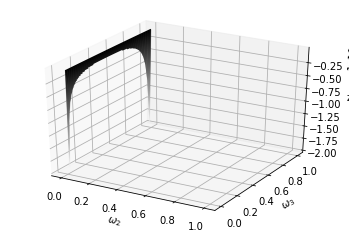
\includegraphics[width=0.49\textwidth]{Chapter4/img/0-01.png}
    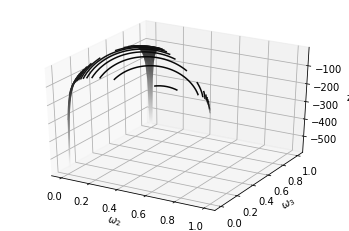
\includegraphics[width=0.49\textwidth]{Chapter4/img/pi-4.png}
    \caption{grid search for different $\alpha$, left: $\alpha=0.01$, right:$\alpha=\pi/4$}
    \label{fig:grid}
\end{figure}

\subsection{A simple first-order method}

Both \XYA~\citep{soare2014linear} and \RAGE~\citep{fiez2019transductive} require to solve an optimization problem of type
\begin{align}\label{eq:fw1}
    \inf_{\bomega\in\Sigma_K} \max_{\bx,\bx'\in\cX} \normm{\bx-\bx'}^2_{\Lambda_{\bomega}^{-1}},
\end{align}
which can be solved by a Frank-Wolfe-typed algorithm applied on the dual problem of~\eqref{eq:fw1} (see e.g.~\citealt{ahipasaoglu2008fw}).

One may notice that the optimization problem that we want to tackle here is of a similar fashion,
\[
    \inf_{\bomega\in\Sigma_K} \max_{\bx,\bx'\in\cX} \frac{\normm{\bx - \bx'}^2_{\Lambda_{\bomega}^{-1}}}{(\bx\transpose\btheta^\star-(\bx')\transpose\btheta^\star)^2}.
\]
It is thus interesting to investigate its dual problem as well. A heuristic is proposed by Degenne et al. (2020) as shown in Algorithm~\ref{alg:solver}, where $\cY$ is defined as \[
    \cY \eqdef \left\{ \frac{(\bx^\star- \bx)}{\left|(\bx^\star-\bx)\transpose\btheta^\star\right|}: \bx\in\cX/\big\{\bx^\star\big\}  \right\}\,.
\]

\begin{algorithm}[ht]
\centering
\caption{Saddle Frank-Wolfe heuristic for computing the optimal weights.}
\label{alg:solver}
\begin{algorithmic}[1]
   \State {\bfseries Input:} arm set $\cX\subset\R^d$, maximum iterations $n$
   \State  {\bfseries Initialize:} $\bomega \leftarrow{} (1, 1, \ldots, 1)\in\R^K, \mathbf{\tLambda} \leftarrow{} I_d, \mathbf{\Lambda}\leftarrow{} I_d, t \leftarrow{} 0$
   \While{$t<n$}
        \State $\mathbf{\tx}\in\argmax_{\bx\in\cX}  \norm{\bx}_{\mathbf{\Lambda}^{-1} \mathbf{\tLambda} \mathbf{\Lambda}^{-1} }^2$
        \State $\mathbf{\ty}\in\argmax_{\by\in\cY}\normm{\by}^2_{\mathbf{\Lambda}^{-1}}$
        \State $\mathbf{\Lambda}\leftarrow{} \mathbf{\Lambda}+ \mathbf{\tx}\mathbf{\tx}\transpose$
		\State $\mathbf{\tLambda} \leftarrow{} \mathbf{\tLambda} + \mathbf{\ty}\mathbf{\ty}\transpose$
        \State $\bomega \leftarrow{} \frac{t}{t+1}\bomega + \frac{1}{t+1}\be_{\mathbf{\tx}}$
        \State $t \leftarrow{} t+1$
   \EndWhile
   \State \Return $\bomega$
\end{algorithmic}
\end{algorithm}